\documentclass[10pt,a4paper]{report}
\usepackage[utf8]{inputenc}
\usepackage[francais]{babel}
\usepackage[T1]{fontenc}
\usepackage{amsmath}
\usepackage{amsfonts}
\usepackage{amssymb}
\usepackage{makeidx}
\usepackage{perpage}
\usepackage{graphicx}
\graphicspath{{Figures/}}
\usepackage[table]{xcolor}
\usepackage{longtable}
\usepackage[tight]{shorttoc}
\usepackage{array}
\usepackage{float}
\usepackage[left=2cm,right=2cm,top=2cm,bottom=2cm]{geometry}

\usepackage{fancyhdr}
\pagestyle{fancy}
\chead{HSMS Software Requirements Specification}
\rhead{}
\lhead{
\includegraphics[width=1.5cm]{logoEseo}}
\cfoot{\thepage}
\rfoot{}
\lfoot{}
{
\renewcommand{\arraystretch}{1.2}
\newcommand{\sommaire}{\shorttoc{Sommaire}{1}} 

\author{L2GB Inc\\
		ESEO option ASTRE\\
		l2gb.inc@gmail.com
		}

\title{HSMS\\Heating Smart Managing Software  \\Software Requirements Specification\\L2GB}


\makeindex
\MakePerPage{footnote}

\usepackage{hyperref} %Pour rendre les références clickable and linkable
\hypersetup{
	colorlinks,
	citecolor=black,
	filecolor=black,
	linkcolor=black,
	urlcolor=black
}

\setcounter{secnumdepth}{5} % Pour que les sections jusqu'au niveau 5 (paragraphe) soient numérotées

\makeindex

\begin{document}

\renewcommand{\figurename}{Illustration} 

\maketitle

\sommaire

	\chapter{Introduction}
		\section{Objet}
		
Ce dossier de spécifications a pour objectif de définir les fonctionnalités et exigences attendues par M. Plainchault pour le développement de la partie logiciel du prototype d'HEMS\footnote{Home Energy Management System} %TODO

Ce document permettra à l'équipe de conception, de réalisation et de tests de concevoir, développer et tester la partie software du prototype.\\

Il pourra également fournir une base pour la planification du développement ainsi qu'à l'estimation des différents coûts qui y sont liés.\\

Les fonctionnalités et exigences présentées dans ce document ont été déterminées suite à l'étude du pfe de 2013 du groupe composé de M Latourte et M Sabatelli \cite{lastPfePoster}.%TODO (référence)
des rencontres et échanges mail avec M. Plainchault, %TODO (référence compte rendu et mail)
des rencontres avec M Delatour, 
des documents relatifs au système Wiser de Schneider  %TODO (référence vers les docs)

Ce document de spécification suit les recommandations de la norme IEE 830-1998 \cite{IEEE_830}. 
Il utilise des schémas et illustrations respectant la norme UML.

		\section{Portée}
		
Ce document décrit les fonctionnalités et exigences du SaE\footnote{Système à l'Etude} constitué:
\begin{description}
	\item[-] De l'application Android Centrale\_Interface permettant à l'utilisateur d'accéder aux relevées de ses consommations et aux scénarios de ses objets connectés qu'il peut également modifier. 
	\item[-] Du logiciel interne Central\_Soft embarquée sur la carte Raspberry Pi gérant la communication entre les objets connectés et le système d'information et permettant la mise en application des scénarios respectifs des dits objets.
\end{description}
\newpage

	\chapter{Description générale}
	
Le SaE est un prototype d'HEMS permettant d'effacer les pointes de consommations énergétiques en agissant directement auprès du consommateur. Le SaE devra, au même titre qu'un HEMS "standard", appliquer les scénarios saisis par l'utilisateur mais devra en plus permettre le lissage des pointes de consommations énergétiques.
Pour cela le SaE devra interagir avec un système d'information en ligne regroupant l'ensemble des données\footnote{Scénarios et relevés des différents capteurs (température extérieur, température des pièces, consommation des prises, ....)} des utilisateurs du système, les relevées météorologiques et les courbes de consommations nationales. \'A partir de ces informations le système d'information recalcule les scénarios des utilisateurs afin de procéder à des reports de consommation tout en respectant leur confort. %TODO s'assurer que ce soit suffisament clair et du coup peut être le modifié si c'est pas le cas

		\section{Caractéristique des acteurs}
	
Par le terme d’acteur, nous désignons toute entité (morale ou physique) qui interagit directement ou non avec le SaE. Cette entité peut être une personne (généralement un utilisateur du système) ou un autre système. Ces acteurs interagissent avec le SaE par intermédiaire des interfaces décrites dans un prochain chapitre.

\begin{description}
	\item[\textbf{L'utilisateur}]: l'utilisateur principal du prototype est le client\footnote{M. Patrick Plainchault}, il ne s’en sert que pour valider l'adéquation entre le système et ses attentes. 
	\item[\textbf{Le système d'information}]: Le système d'information est le serveur en ligne comprenant l’outil big data utilisé.
	\item[\textbf{Le technicien de maintenance}]: Personne chargée du développement et de la maintenance du SaE.
	\item[L'objet connecté]: Tous objets connectés à la centrale : Prises, sonde radiateur etc….
	\item[La Central\_Hard]: Carte électronique et son boitier supportant le logiciel Central\_Soft
\end{description}

		\section{Environnement}
	
La présente section permet de définir la frontière entre le SaE et les différentes entités qui l'environnent.

			\subsection{Architecture matérielle et logicielle}
			
Le diagramme de déploiement de l'illustration~\ref{diagArchiMatSof} page~\pageref{diagArchiMatSof}  représente architecture logicielle et matérielle du SaE. Les conventions graphiques utilisées sont explicitées sur l'illustration~\ref{diagDeploiLegende} page~\pageref{diagDeploiLegende}. 
Ce diagramme de déploiement identifie les entités matérielles et/ou logicielles avec lesquelles le SaE (composé des entités Centrale\_soft, Centrale\_interface) doit interagir et permet ainsi de déterminer les principaux échanges qu'il entretient avec son environnement.

La carte de développement nommée ici E\_Centrale est une carte Rasberry Pi modèle B+ équipé d'un processeur %TODO 
qui communique avec les objets connectés par le biais d'un module Z-Wave et avec l'E\_PC en Ethernet. %TODO référence précise

Cette carte repose sur un système d'exploitation LINUX que nous appelons ici OS\_LINUX\_EMBARQUE dont la version du Kernel est %TODO mettre numéro de version et rajouter OS_LINUX_EMBARQUE sur le diagramme



\begin{figure}[H]
	\centering
	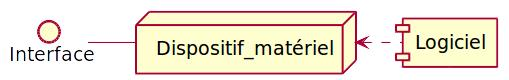
\includegraphics[scale=0.55]{diagDeploiLegende}
	\caption{Légende du diagramme de déploiement}
	\label{diagDeploiLegende}
\end{figure}


\begin{figure}[H]
	\centering
	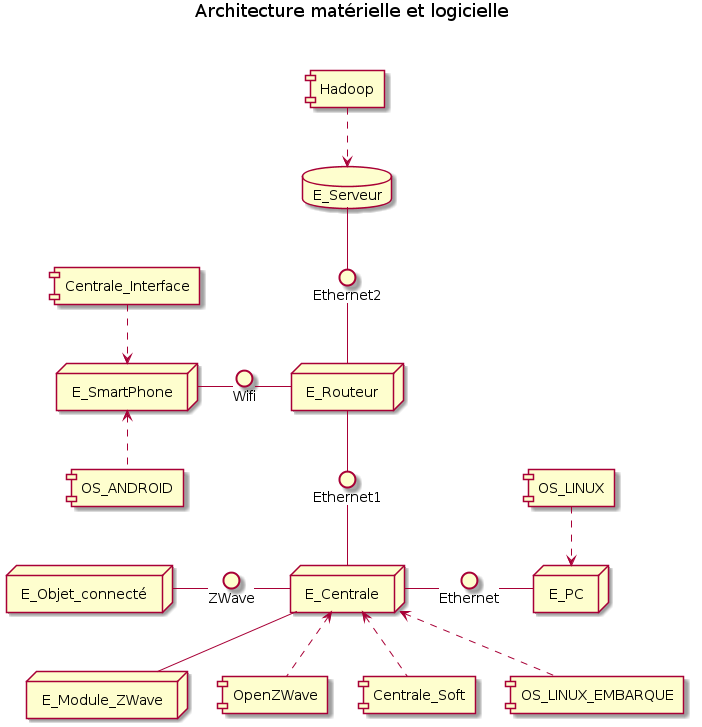
\includegraphics[scale=0.55]{diagArchiMatSof}
	\caption{Diagramme d'architecture matérielle et logicielle}
	\label{diagArchiMatSof}
\end{figure}
%TODO rajouter OS_LINUX_EMBARQUE, remplacer Big_Data par Hadoob et sa version ou quelque chose comme ça, d'ailleurs sur le schéma regarder pourquoi y a Big_data ET E_BigData, mettre la version de l'OS qui est sur E_PC ainsi que la version de son noyau si c'est du linux, et possiblement aussi du coup mettre la librairie open z-wave 

L'E\_Routeur correspond à la Box internet de l'utilisateur.
\newpage

			\subsection{Interface du système}
		
Ce chapitre décrit les entrées/sorties du système avec les différents acteurs interagissant avec lui. \\

On peut différencier deux grands types d’entrées/sorties, celles dites de « haut niveau » (également nommées entrées/sorties logiques) qui décrivent les interactions avec les utilisateurs (client et technicien de maintenance) et celles de « bas niveau » (ou physiques) correspondant aux données réellement échangées entre le système et ses périphériques.

			\subsection{Les interfaces avec les utilisateurs}
			
Il y a deux utilisateurs du système : le client (également nommé utilisateur par la suite) et le technicien de maintenance (ou développeur). Le client interagit avec le système via une page web (« L2GB Manager »). Le technicien quant à lui peut également se connecter en interface directe à la carte raspberry présente sur la centrale via un ordinateur. (cf. description de l’architecture matérielle du système pour plus de détails).\\

Ces deux utilisateurs ont été présentés avec les acteurs.\\

Les évènements énoncés ci-dessous sont d’ordre logique, ils correspondent à une interprétation par le SaE d’évènements physiques de plus bas niveau décrits plus loin.			


	\chapter{Contexte logique}
	
\begin{figure}[H]
	\centering
	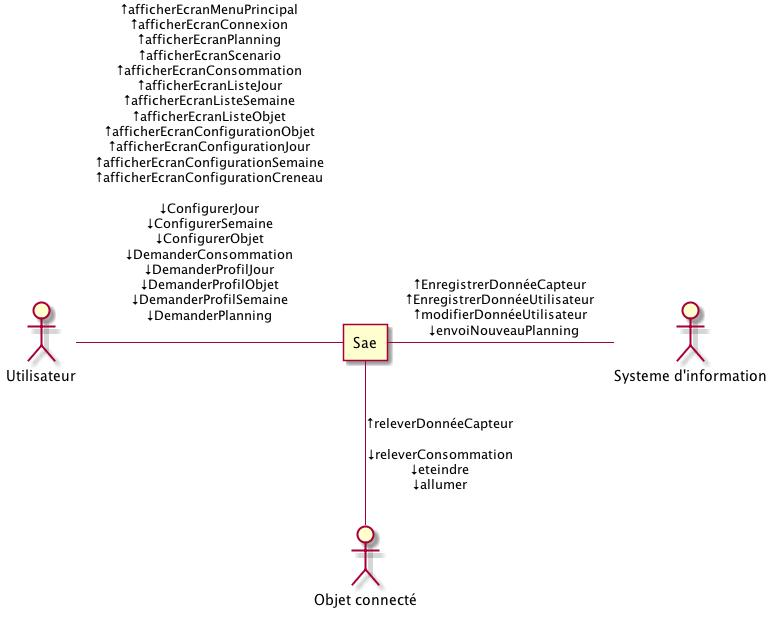
\includegraphics[scale=0.55]{diagContexteLogique}
	\caption{Diagramme de contexte logique}
	\label{diagContexteLogique}
\end{figure}
\newpage

		\section{Interface logique avec l'utilisateur}
			\subsection{En provenance de l'utilisateur vers le SaE}
			
\begin{description}
	\item[-] ConfigurerJour: Permet à l'utilisateur de configurer un jour.
	\item[-] ConfigurerSemaine: Permet à l'utilisateur configurer une semaine.
	\item[-] ConfigurerObjet: Permet à l'utilisateur de configurer un objet.
	\item[-] DemanderConsommation: Permet à l'utilisateur de voir la consommation de ses objets.
	\item[-] DemanderProfilJour: Permet à l'utilisateur d'afficher ses profils jours enregistrés
	\item[-] DemanderProfilSemaine: Permet à l'utilisateur d'afficher ses profils semaine 
	\item[-] DemanderProfilObjet: Permet à l'utilisateur d'afficher les objets connectés 
	\item[-] DemanderPlanning: Permet à l'utilisateur d'afficher le planning global des objets de sa maison
	
	
\end{description}
			
			\subsection{En provenance du SaE vers l'utilisateur}
			
\begin{description}
	\item[-] afficherEcranMenuPrincipal: affiche le menu principal du site
	\item[-] afficherEcranConnexion: affiche l'écran de connexion du site 
	\item[-] afficherEcranPlanning: affiche l'écran de planning
	\item[-] afficherEcranScenario: affiche l'écran scénario
	\item[-] afficherEcranConsommation: affiche l'écran listant la consommation des différents objets connectés
	\item[-] afficherEcranListeJour: affiche l'écran des profils jours enregistrés
	\item[-] afficherEcranListeSemaine: affiche l'écran des profils semaine enregistrés
	\item[-] afficherEcranListeObjet: affiche l'écran des objets enregistrés
	\item[-] afficherEcranConfigurationObjet: affiche l'écran de configuration des objets.
	\item[-] afficherEcranConfigurationJour: affiche l'écran de configuration des jours.
	\item[-] afficherEcranConfigurationSemaine: affiche l'écran de configurations des semaines.
	\item[-] afficherEcranConfigurationCreneau: affiche l'écran pour configurer un créneau horaire.
\end{description}
			
		
		\section{Interface logique avec le système d'information}
			\subsection{En provenance du système d'information vers le SaE}
			
\begin{description}
	\item[-] EnregistrerDonnéeCapteur: stocke les données des capteurs sur la big data.
	\item[-] EnregistrerDonnéeUtilisateur: Stocke les données de l'utilisateur sur la big data.
	\item[-] modifierDonnéeUtilisateur: Modifie les données utilisateur sur la big data.
	
\end{description}
			
			\subsection{En provenance du SaE vers le système d'information}
			
\begin{description}
	\item[-] envoiNouveauPlanning: Envoie un nouveau planning d'utilisation aux objets
\end{description}
			
			
		\section{Interface logique avec un objet connecté}
			\subsection{En provenance de l'objet connecté vers le SaE}
			
\begin{description}
	\item[-] releverDonneeCapteur: Envoie des données de l'objet connecté à la centrale.
\end{description}
			
			\subsection{En provenance du SaE vers l'objet connecté}
			
\begin{description}
	\item[-] releverConsommation: Demande la consommation d'un objet à l'instant T
	\item[-] éteindre: Demande à l'objet de se mettre sur off.
	\item[-] allumer: Demander à l'objet de se mettre sur on.
\end{description}


	\chapter{Cas d'utilisation}
		\section{Conventions cas d'utilisation}

{
\renewcommand{\arraystretch}{1.2}
\begin{longtable}{| p{5cm} | p{11cm} |}
	\hline
	\cellcolor{lightgray}\textbf{\textbf{Titre}} & \cellcolor{lightgray}\textbf{Rappel en quelques mots l'objectif principal du CU}\tabularnewline
	\hline
	\textbf{Résumé} & Décrit brièvement le comportement du CU.\tabularnewline
	\hline
	\textbf{Portée} & Définit la portée de conception du CU.\tabularnewline
	\hline
	\textbf{Niveau} & Niveau de granularité du CU\footnote{Stratégique, utilisateur ou sous-fonction}\tabularnewline
	\hline
	\textbf{Acteurs} & Le premier déclenche le CU, les autres y participent\tabularnewline
	\hline
	\textbf{Préconditions } & Ensemble des conditions qui doivent être vérifiées avant le déroulement du CU. Les préconditions, sans mention contraire explicite, des CUs parents aux CUs fils doivent toujours être vérifiées.\tabularnewline
	\hline
	\textbf{Garanties minimales} & Définis ce qui est garanti par le SaE même en cas d'échec du CU.\tabularnewline
	\hline
	\textbf{Garantie en cas de succès} & Définis les garanties en cas de succès ( par le scénario nominal ou par ses variantes).\tabularnewline
	\hline
	\textbf{Scénario nominal} & C'est un scénario représentatif de l'utilisation du système où tout se passe bien. Il se termine par la réussite des objectifs. Il est constitué d'une condition déclenchant le scénario, d'un ensemble d'étapes, d'une condition de fin et éventuellement d'extensions ou de variantes. Une étape peut être une interaction entre acteurs ou une étape de validation.\tabularnewline
	\hline
	\textbf{Variantes} & Lorsqu'il y a plusieurs façons de procéder à une même étape sans remise en cause du scénario nominal.\tabularnewline
	\hline
	\textbf{Extensions} & Définissent les autres scénarios que le scénario nominal (par exemple ceux qui se terminent par un échec). Elles se déclenchent sur des conditions spécifiques détectées par le SaE.\tabularnewline
	\hline
	\textbf{Informations complémentaires} & Informations diverses nécessaires à la compréhension du CU.\tabularnewline
	\hline
\caption{Convention utilisée pour la présentation des CUs}	
\label{tableConventionCU}
\end{longtable}
}

		\section{Cas d'utilisation Contrôler la Consommation}

\begin{figure}[H]
	\centering
	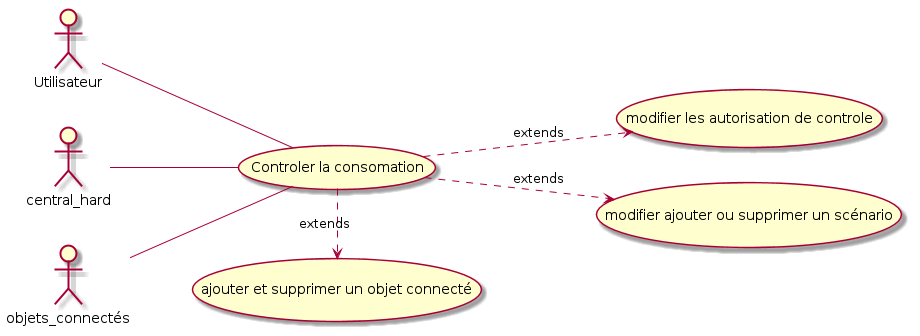
\includegraphics[scale=0.55]{diagCU_ControlerConso}
	\caption{Diagramme de cas d'utilisation Contrôler Consommation}
	\label{diagCuControlerConso}
\end{figure}

{
\renewcommand{\arraystretch}{1.2}
\begin{longtable}{| p{5cm} | p{11cm} |}
	\hline
	\cellcolor{lightgray}\textbf{\textbf{Titre}} & \cellcolor{lightgray}\textbf{Contrôler la consommation}\tabularnewline
	\hline
	\textbf{Résumé} & Ce cas d'utilisation représente la séquence d'utilisation du SaE par l'utilisateur.\tabularnewline
	\hline
	\textbf{Portée} & L'ensemble du SaE.\tabularnewline
	\hline
	\textbf{Niveau} & Stratégique\tabularnewline
	\hline
	\textbf{Acteurs} & Utilisateur, Système d'Information, Objets connectés\tabularnewline
	\hline
	\textbf{Préconditions } & Le code est chargé sur la cible, Central\_Hard est sous tension.\tabularnewline
	\hline
	\textbf{Garanties minimales} & \tabularnewline
	\hline
	\textbf{Garantie en cas de succès} & \tabularnewline
	\hline
	\textbf{Scénario nominal} & \begin{description}
		\item[1.] L'utilisateur démarre la Central\_Hard
		\item[2.] L'utilisateur se connecte 
		\item[3.] Central\_Soft affiche son écran "Connexion"
		\item[4.] L'utilisateur s'authentifie
		\item[5.] Central\_Soft affiche son écran "Accueil"
		\item[6.] L'utilisateur se déconnecte
	\end{description} \tabularnewline
	\hline 
	\textbf{Variantes} &\begin{description}
		\item[6:] [L'utilisateur veut modifier/supprimer/ajouter un scénario]
		\item[6.a.1] L'utilisateur choisit d'accéder à la configuration des scénarios
		\item[6.a.2] Central\_Soft affiche son écran "Scénario"
		\item[6.a.3] L'utilisateur choisit le scénario à modifier/supprimer/ajouter
		\item[6.a.4] L'utilisateur modifie/supprimer/ajoute le scénario choisi
		\item[6.a.5] L'utilisateur confirme la modification/suppression/ajout
		\item[6.a.6] L'utilisateur choisit de revenir à l'accueil
		\item[6.a.7] Retour en 5
	\end{description} 
	---------------------------------------------------------------------------------------------
	\begin{description}
		\item[6:] [L'utilisateur veut ajouter/supprimer un objet connecté]
		\item[6.b.1] L'utilisateur choisit d'accéder à la configuration des objets connectés
		\item[6.b.2] Central\_Soft affiche son écran "Objets connectés"
		\item[6.b.3] L'utilisateur choisit l'objet connecté à supprimer/ajouter
		\item[6.b.4] L'utilisateur supprime/ajoute l'objet
		\item[6.b.5] L'utilisateur confirme la suppression/ajout 
		\item[6.b.6] L'utilisateur choisit de revenir à l'accueil
		\item[6.b.7] Retour en 5
	\end{description}
	---------------------------------------------------------------------------------------------
	\begin{description}
		\item[6:] [L'utilisateur veut modifier les autorisations de contrôle]
		\item[6.c.1] L'utilisateur choisit d'accéder à la configuration des autorisations de contrôle
		\item[6.c.2] Central\_Soft affiche son écran "Objets connectés"
		\item[6.c.3] L'utilisateur choisit les autorisation de contrôle à modifier
		\item[6.c.4] L'utilisateur modifie cette dernière
		\item[6.c.5] L'utilisateur confirme la modification
		\item[6.c.6] L'utilisateur choisit de revenir à l'accueil
		\item[6.c.7] Retour en 5
	\end{description}\tabularnewline
	\hline
	\textbf{Extensions} & Définissent les autres scénarios que le scénario nominal (par exemple ceux qui se terminent par un échec). Elles se déclenchent sur des conditions spécifiques détectées par le SaE.\tabularnewline
	\hline
	\textbf{Informations complémentaires} & Informations diverses nécessaires à la compréhension du CU.\tabularnewline
	\hline
\caption{Cas d'utilisation Contrôler la consommation}	
\label{tableUC_ControlerConso}
\end{longtable}
}

		\section{Cas d'utilisation Modification Automatique d'un Scénario}

\begin{figure}[H]
	\centering
	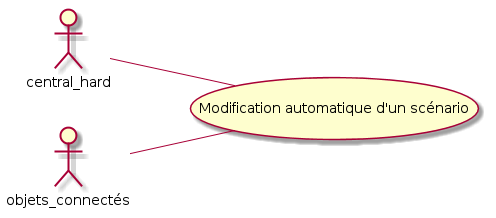
\includegraphics[scale=0.55]{diagCU_ModifAutoScenar}
	\caption{Diagramme de cas d'utilisation Modification automatique d'un scénario}
	\label{diagCuModifAutoScenar}
\end{figure}

{
\renewcommand{\arraystretch}{1.2}
\begin{longtable}{| p{5cm} | p{11cm} |}
	\hline
	\cellcolor{lightgray}\textbf{\textbf{Titre}} & \cellcolor{lightgray}\textbf{Contrôler la consommation}\tabularnewline
	\hline
	\textbf{Résumé} & Ce cas d'utilisation représente la séquence de fonctionnement du SaE sans intervention de l'utilisateur.\tabularnewline
	\hline
	\textbf{Portée} & L'ensemble du SaE.\tabularnewline
	\hline
	\textbf{Niveau} & Stratégique\tabularnewline
	\hline
	\textbf{Acteurs} & Système d'Information, Objets Connectés\tabularnewline
	\hline
	\textbf{Préconditions } & Le code est chargé sur la cible, Central\_Hard est sous tension\tabularnewline
	\hline
	\textbf{Garanties minimales} & \tabularnewline
	\hline
	\textbf{Garantie en cas de succès} & Les objet connecté reçoivent les ordres de la centrale selon les consignes envoyées au système d'information\tabularnewline
	\hline
	\textbf{Scénario nominal} & \begin{description}
		\item[1.] Le système d'information envoie des nouveaux planning de consommation.
		\item[2.] La Central\_Soft met en application les nouveaux scénarios
	\end{description}\tabularnewline
	\hline 
	\textbf{Variantes} & \tabularnewline
	\hline
	\textbf{Extensions} & \tabularnewline
	\hline
	\textbf{Informations complémentaires} & L'envoie des consommations des différents objets connectés sont envoyés en parallèle au système\tabularnewline
	\hline
\caption{Cas d'utilisation Modification automatique d'un scénario}	
\label{tableUC_ModifAutoScenar}
\end{longtable}
}

Comme indiqué sur l'illustration~\ref{diagArchiMatSof} page~\pageref{diagArchiMatSof}, la Centrale (représenté au centre) est en interaction avec différentes entités externes au SaE. Par convention, le nom de ces entités est préfixé par les lettre "E\_" (E pour Externe), elles sont aussi désignées, dans ce document, par le terme de "périphérique Centrale". \\

Pour les besoins classiques de développement et de maintenance (téléchargement, débogage et diagnostic), une liaison Ethernet avec un ordianteur devra être prévue.\\

La liste des périphériques Centrale est donc la suivante:

\begin{description}
	\item[\textbf{\textperiodcentered}] E\_Centrale: Carte à micro-processeur de type Raspberry Pi équipée d'un linux embarqué.
	\item[\textbf{\textperiodcentered}] E\_Module\_ZigBee: Module ZigBee permettant l'émission et la réception de trames respectant le protocole ZigBee.
	\item[\textbf{\textperiodcentered}] E\_Objet\_Connecté: %TODO
	\item[\textbf{\textperiodcentered}] E\_PC: Il s'agit de n'importe quel ordinateur possédant un port Ethernet permettant de se connecter à la Centrale. Ce périphérique n'est utilisé que par les techniciens de maintenance et/ou développeurs et en aucun cas par le client.
	\item[\textbf{\textperiodcentered}] E\_Routeur: Point d'accès à internet sur lequel on peut se connecter en Wifi ou en Ethernet.
	\item[\textbf{\textperiodcentered}] E\_Serveur: Plateforme permettant d'heberger le BigData.
\end{description}

	\chapter{IHMs logiques}
	
		\section{Accueil}
	
\begin{figure}[H]
	\centering
	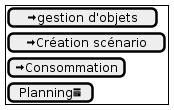
\includegraphics[scale=0.55]{Accueil}
	\caption{IHM logique "Accueil"}
	\label{ihmLogiqueAccueil}
\end{figure}

		\section{Choix objet}

\begin{figure}[H]
	\centering
	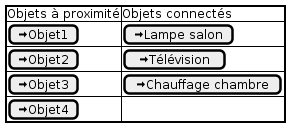
\includegraphics[scale=0.55]{Choix_objet}
	\caption{IHM logique "Choix objet"}
	\label{ihmLogiqueChoixObjet}
\end{figure}

		\section{Ajout Objet}

\begin{figure}[H]
	\centering
	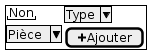
\includegraphics[scale=0.55]{Objet_Ajout}
	\caption{IHM logique "Objet Ajout"}
	\label{ihmLogiqueObjetAjout}
\end{figure}

		\section{Identification}

\begin{figure}[H]
	\centering
	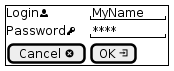
\includegraphics[scale=0.55]{Identification}
	\caption{IHM logique "Identification"}
	\label{ihmLogiqueIdentification}
\end{figure}

		\section{Modification profil objet}

\begin{figure}[H]
	\centering
	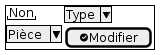
\includegraphics[scale=0.55]{Objet_profil_modif}
	\caption{IHM logique Modification Profil Objet"}
	\label{ihmLogiqueObjProModif}
\end{figure}

		\section{Objet profil}

\begin{figure}[H]
	\centering
	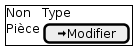
\includegraphics[scale=0.55]{Objet_profil}
	\caption{IHM logique "Profil"}
	\label{ihmLogiqueProfil}
\end{figure}

		\section{Consommation}

\begin{figure}[H]
	\centering
	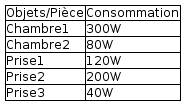
\includegraphics[scale=0.55]{Consommation}
	\caption{IHM logique "Consommation"}
	\label{ihmLogiqueConso}
\end{figure}

		\section{Semaine}

\begin{figure}[H]
	\centering
	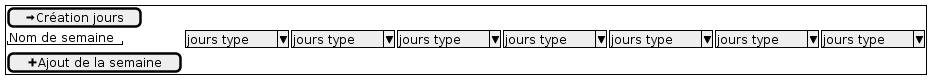
\includegraphics[scale=0.55]{Semaine}
	\caption{IHM logique "Semaine"}
	\label{ihmLogiqueSemaine}
\end{figure}

		\section{Mois}

\begin{figure}[H]
	\centering
	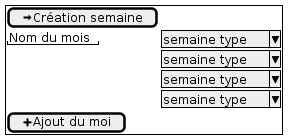
\includegraphics[scale=0.55]{Mois}
	\caption{IHM logique "Mois"}
	\label{ihmLogiqueMois}
\end{figure}

		\section{Jours}

\begin{figure}[H]
	\centering
	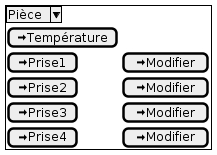
\includegraphics[scale=0.55]{Jours}
	\caption{IHM logique "jours"}
	\label{ihmLogiqueJours}
\end{figure}

	\chapter{Dictionnaire domaine}
	
{
\renewcommand{\arraystretch}{1.2}		
\begin{longtable}{| l | p{11cm} |}
	\hline
	\textbf{Terme} & Définition\tabularnewline
	\hline
	\textbf{Autorisation de contrôle} & Autorisation permettant la modification ou non des scénarios par la centrale des scénarios prédéfinit par l'utilisateur\tabularnewline
	\hline
	\textbf{Central\_Hard} & Carte électronique et boitier permettant la communication avec les objets connectés et le système d'information\tabularnewline
	\hline
	\textbf{Central\_Soft} & Logiciel qui s'exécute sur la Central\_Hard \tabularnewline
	\hline
	\textbf{Consigne de consommation} & fonction envoyée par le SI au SaE\tabularnewline
	\hline
	\textbf{Home Energy Management System} &  \tabularnewline%TODO
	\hline
	\textbf{Objet connecté} & Carte électronique et boitier permettant d'allumer ou éteindre une alimentation \tabularnewline %TODO WTF
	\hline
	\textbf{Ordre de consommation} & Fonction envoyée du SaE aux objets connectés\tabularnewline
	\hline
	\textbf{Scénario} & Programmation du fonctionnement d'un objet connecté en fonction de l'heure, du jour et de la semaine\tabularnewline
	\hline
	\textbf{Système d'information} & Système hébergé sur internet qui permet de recueillir les données de consommation de la Centrale et de lui envoyer les consignes de consommation\tabularnewline
	\hline
\caption{Dictionnaire domaine}
\label{dicoDomaine}
\end{longtable}
}

\bibliographystyle{plain}
\bibliography{bibliography}	

\tableofcontents
\listoffigures
\listoftables

\end{document}